\chapter{Population Variation in the Associations Between Large-Scale Networks and Experiences at Rest}
\chaptermark{Large-scale network and experiences}
\label{ch:study2}
%\setcounter{equation}{0}

% ==========================================================================================================

\textit{The following chapter has been adapted from: }Wang, H.-T., Bzdok, D., Margulies, D., Craddock, C., Milham, M., Jefferies, E., \& Smallwood, J.(2018). Patterns of thought: Population variation in the associations between large-scale network organisation and self-reported experiences at rest.
\textit{NeuroImage}, \textit{176} (1), 518--527. doi: \url{10.1016/j.neuroimage.2018.04.064} \footnote{
J. Smallwood, and H.-T. Wang designed the study. The data was provided from C. Cameron and M. Milham. The analysis pipeline was constructed by H.-T. Wang under the supervision of D. Bzdok and J. Smallwood. Data were analyzed by H.-T. Wang, under the supervision of D. Bzdok, J. Smallwood, and E. Jefferies. H.-T. Wang and J. Smallwood drafted the manuscript. D. Bzdok, D. Margulies and E. Jefferies provided critical input to the interpretations. All the authors approved the final version of the manuscript prior to submission.}

% ==========================================================================================================

\section{Abstract}
Contemporary cognitive neuroscience recognises unconstrained processing varies across individuals, describing variation in meaningful attributes, such as intelligence. It may also have links to patterns of ongoing experience. This study examined whether dimensions of population variation in different modes of unconstrained processing can be described by the associations between patterns of neural activity and self-reports of experience during the same period. We selected 258 individuals from a publicly available data set who had measures of resting-state functional magnetic resonance imaging, and self-reports of experience during the scan. We used machine learning to determine patterns of association between the neural and self-reported data, finding variation along four dimensions. `Purposeful' experiences were associated with lower connectivity---in particular default mode and limbic networks were less correlated with attention and sensorimotor networks. `Emotional' experiences were associated with higher connectivity, especially between limbic and ventral attention networks. Experiences focused on themes of `personal importance' were associated with reduced functional connectivity within attention and control systems. Finally, visual experiences were associated with stronger connectivity between visual and other networks, in particular the limbic system. Some of these patterns had contrasting links with cognitive function as assessed in a separate laboratory session---purposeful thinking was linked to greater intelligence and better abstract reasoning, while a focus on personal importance had the opposite relationship. Together these findings are consistent with an emerging literature on unconstrained states and also underlines that these states are heterogeneous, with distinct modes of population variation reflecting the interplay of different large-scale networks.

% ====================================================================================================================
\section{Introduction}
\label{study2:intro}
Unconstrained processing reflects important population level variation in measures of cognition, affect, and demographic \/ lifestyle factors. Psychological studies show that almost a third of ongoing thought is unconstrained by events in the here-and-now \cite{Killingsworth2010}
with important links to cognitive and affective processing \cite{Mooneyham2013}.
In neuroscience, metrics defined from the brain during wakeful rest, describe the organisation of neural function at both the micro and macro scale \cite{Glasser2016,Margulies2016}.
They also reflect individual differences in cognitive function \cite{Finn2015},
psychiatric conditions \cite{Nooner2012}
and demographic \/ lifestyle factors \cite{Smith2015}.
These findings establish unconstrained neurocognitive processing as a core element of human cognition, highlighting the need to formally understand the underlying neural architecture, and the associated patterns of experience.

One perspective on unconstrained processing emphasises the role of memory, with contributions of conceptual and episodic representations to ongoing thought \cite{Binder2009,Gusnard2001}.
Psychological studies have shown that patterns of unconstrained processing have links with memory retrieval, creativity and planning \cite{Baird2012,Leszczynski2017,Medea2016,Poerio2017}.
Such evidence raises the possibility that episodic representations anchored in the medial temporal lobe \cite{Moscovitch2016}
or conceptual representation anchored in anterior temporal lobe \cite{Lambon-Ralph2017}
contribute to ongoing thought \cite{Smallwood2016}.
It is hypothesised that these systems' contribution to unconstrained states may be linked to the ability for these regions to become functionally decoupled from systems more directly involved in action and perception, allowing them to operate in an offline manner \cite{SmallwoodCC2013}.
This process of decoupling may also be important in neural systems closely allied to those involved in memory – the default mode network \cite{Raichle2001}.
These regions of transmodal cortex are relatively distant in functional and structural space from systems involved in perception and action, potentially facilitating their role in stimulus independent aspects of cognition \cite{Buckner2013,Margulies2016,Mesulam1998}.
Together these \textit{representational} accounts of unconstrained processing highlight default mode and limbic networks as important candidate neural systems, especially when decoupled from systems directly involved in perception and action.

Alternative perspectives on unconstrained thought emerge from links between types of ongoing experience and problems maintaining a task relevant goal in mind. This \textit{executive-failure} view \cite{Kane2012,McVay2009}
takes as a starting point evidence that patterns of ongoing thought, such as the experience of mind-wandering, are linked to problems on tasks including sustained attention \cite{McVay2009}
and measures of general aptitude and executive control \cite{MrazekJoEP2012}.
Task-based neuroimaging investigations highlight a network of regions that increase their activity across many different task situations, so called multiple demand regions \cite{Duncan2010}. %(Duncan, 2010).
These regions broadly correspond to three well described intrinsic networks: ventral attention, dorsal attention, and frontal-parietal networks. Since these systems are important for the effective performance of many different tasks then dysregulation within these systems could reflect the hypothesised \textit{executive-failure} contribution to aspects of ongoing thought \cite{McVay2009,Weissman2006}.%(McVay \& Kane, 2010; Weissman, Roberts, Visscher, \& Woldorff, 2006).

Other aspects of unconstrained processing could reflect the importance of affective processes, or different modalities of processing. Ongoing thought is linked to mood state: Experimental inductions of mood \cite{SmallwoodEmotion2009,Smallwood2011}
%(Smallwood, Fitzgerald, Miles, \& Phillips, 2009; Smallwood \& O'Connor, 2011)
as well as natural fluctuations \cite{Poerio2013, RubyPlos2013}
%(Poerio, Totterdell, \& Miles, 2013; Ruby, Smallwood, Engen, \& Singer, 2013)
impact on ongoing thought. Contemporary accounts of emotional processing emphasise the role of limbic regions including the amygdala \cite{Bzdok2013,Lindquist2012}
%(Bzdok, Laird, Zilles, Fox, \& Eickhoff, 2013; Lindquist, Wager, Kober, Bliss-Moreau, \& Barrett, 2012)
and anterior aspects the insula \cite{Touroutoglou2012},
%(Touroutoglou, Hollenbeck, Dickerson, \& Barrett, 2012),
suggesting these regions may be important in determining affective aspects of ongoing thought. Psychological studies of ongoing thought also suggest that another important dimension of unconstrained processing may reflect the different modalities of processing \cite{Konishi2017,Smallwood2016}.
%(Konishi, Brown, Battaglini, \& Smallwood, 2017; Smallwood et al., 2016).
It has been shown, for example, that the visual system plays an important role in the expression of visual imagery \cite{Ganis2004,Kosslyn2001}.
%(Ganis, Thompson, \& Kosslyn, 2004; Kosslyn, Ganis, \& Thompson, 2001).
Recent work has extended this evidence to shown patterns of activity with visual regions are linked to the emergence of visual, non-verbal, elements of ongoing thought \cite{Raij2017}.
%(Raij \& Riekki, 2017).
It is also possible that sensorimotor processes may be implicated in language processing during unconstrained processing, given that a role for these regions in langauge processing extends beyond production \cite{Bzdok2016,Pulvermuller2010,Pulvermuller2010a}.
%(Bzdok et al., 2016; Pulvermuller, 2010; Pulvermuller \& Fadiga, 2010).

Our study aimed to identify patterns of intrinsic connectivity associated with different patterns of unconstrained states and examines their neurocognitive features from the perspectives outlined above. We used a large publicly available dataset, containing measures of resting-state functional magnetic resonance imaging (fMRI), and an accompanying self-report instrument describing cognition experienced during the resting state \cite{Gorgolewski2014,Nooner2012}. We previously explored the relationships between patterns of ongoing thought and measures of neural activity, such as the fractional amplitude of low frequency oscillations, as well as the regional homogeneity of neural activity, in a sub sample of this data set \cite{Gorgolewski2014}. In this study we focused on connectivity, we applied sparse canonical correlation analysis (SCCA) to obtain a conjoined decomposition of self-reports of experience with matrices of whole brain connectivity data. This analysis produces multivariate patterns that reflect dimensions of variation that are mutually constrained by both brain and experience. In this way we capitalise on the fact that self-reports of experience during scanning and descriptions of ongoing neural processing provide complementary descriptions of unconstrained cognition. Our analysis, therefore, helps define, at a population level, the shared links between brain patterns and different types of experience. Moreover, respecting the multivariate nature of brain and behaviour space, as our analysis does, can accommodate complex many-to-many relationships between patterns of connectivity and self-reports, and therefore is sensitive to the possibility of degeneracy in the underlying data. As a final validation step we established whether these neurocognitive dimensions are associated with performance on a battery of available cognitive tasks, including measures of executive control and intelligence.

We use the dimensions our analysis produces, and their links with cognitive function to evaluate the perspectives on unconstrained thought outlined earlier. \textit{Representational} accounts emphasise links with neural systems involved in memory, such as the limbic system, and regions of transmodal cortex, such as the default mode network. They highlight states with lower levels of functional communication between these regions and those more directly involved in external action. In contrast, \textit{executive-failure} accounts emphasise dysregulation in attention and control networks as contributing to patterns of ongoing thought that are linked to problems in domain general task performance. Affective accounts highlight limbic regions as important hubs in aspects of ongoing thoughts linked to emotion. Finally, modality specific influences on unconstrained thought may depend on information codes represented in regions that specialise in that particular type of information, such as a role of visual cortex in experiences dominated by images. Notably, some views lead to dissociable predictions with respect to cognitive performance. For example, executive-failure accounts predict patterns of thoughts linked to worse performance on measures of cognitive function, while representational accounts makes the opposite prediction.
% ==========================================================================================================

\section{Method}
\label{study2:method}

\subsection{Participants}
\label{study2:method:participants}
We analysed 258 participants (females = 162; age range 18 –- 55, \textit{M} = 34.97, \textit{SD} = 12.24) obtained from the enhanced Nathan Kline Institute-Rockland sample (NKI-RS;  \url{http://fcon_1000.projects.nitrc.org/indi/enhanced/}).
Full details of the acquisition of this sample can be found in \citeA{Nooner2012}.
We selected participants between 18 and 55 years old as our sample, this choice allowed us to maximise the cohesive nature of our sample.  All the participants have the MRI data and less than 5 missing data points among the selected assessments.

\subsection{Cognitive measures and questionnaires}
\label{study2:method:cog}
Based on prior studies examining the links between spontaneous thought and cognitive performance \cite<see>{Mooneyham2013}, %(see Mooneyham \& Schooler, 2013)
we selected established neuropsychological measures linked to executive control, abstract reasoning and intelligence. The measures included the Delis-Kaplan Executive Function System \cite<D-KEFS;>{Swanson2005},
Wechsler Abbreviated Scale of Intelligence \cite<WASI-II;>{Wechsler1999},
and Wechsler Individual Achievement Test-Second Edition Abbreviated \cite<WIAT-IIA;>{Wechsler2005}.
In D-KEFS we selected the tower test (move accuracy ratio), colour-word interference test (errors inhibition\(/\)switching), verbal fluency test (letter fluency \(-\) category fluency), design fluency test (design accuracy), trail making test (sequencing errors score \(+\) set-loss errors score \(+\) time-discontinue errors score), and the proverb test (a measure of abstract semantic reasoning). We used the rescaled score (\textit{M} = 10, \textit{SD} = 3) in our analysis. Tasks measures that reflected error rates (i.e. the colour-word interference test and trail making test) were reversed, so that high rescaled scores indicated better task performance. All the scores were transformed to z-scores.

\subsection{ongoing cognition measure}
\label{study2:method:NYCQ}
The New York Cognition Questionnaire (NYC-Q) is a self-report tool used to assess the thoughts experienced at rest \cite{Gorgolewski2014,Sanders2017}.
%(Gorgolewski et al., 2014; Sanders, Wang, Schooler, \& Smallwood, 2017).
It assesses thoughts and feelings experienced during the resting-state period. The first section contains 23 questions about the content of thought. These questions covers the temporal, social, emotional aspects of spontaneous thoughts that have been shown to be important by prior studies \cite<e.g.>{RubyPlos2013}.
Participants rated each question on a scale of 1 (Completely did not describe my thoughts) to 9 (Completely did describe my thoughts). The second section contains 8 questions about the forms thoughts take, capturing aspects of experience such as modality and detail associated with experience that prior studies suggest as important for spontaneous thoughts \cite{Smallwood2016}.
Participants rated each question on a scale of 1 (Completely did not characterise my experience) to 9 (Completely did characterise my experience).  In the current study we analysed the two sections together to provide single solutions that combined information on both the content form of experience. The full list of questions and the corresponding labels are presented in \cref{tab:study2:1}. The questionnaire was administrated once after the resting-state scan in order to assess experiences during the scanning session. For the full details of the NYC-Q, please refer to \citeA{Gorgolewski2014}.
We have placed the questionnaire measure used in this study along with an example self-report collection task on GitHub at the following address:
\url{https://github.com/htwangtw/restingstate_thoughtreports}.

\linespacesmall

\begin{table}
\centering
\caption{The New York Cognition Questionnaire (NYC-Q).}
\label{tab:study2:1}

\resizebox{\textwidth}{!}{
\begin{tabular}{ l l}
\toprule
Questions&Labels\\
\midrule
I thought about things I am currently worried about&Concerns\\
I thought about people I have just recently met&People\\
I thought of people I have known for a long time (friends)&Friend\\
I thought about members of my family&Family\\
I thought about an event that took place earlier today&Today - Past\\
I thought about an interaction I may possibly have in the future&Social - Future\\
I thought about an interaction with somebody that took place in the past&Social - Past\\
I thought about something that happened at a place very close to me&Near Location\\
I thought about something that made me feel guilty&Guilt\\
I thought about an event that may take place later today&Today - Plan\\
I thought about something that happened in the recent past (last couple of days but not today)&Recent Past\\
I thought about something that happened a long time ago in the past&Distant Past\\
I thought about something that made me angry&Anger\\
I thought about something that made me happy&Happiness\\
I thought about something that made me cheerful&Cheerfulness\\
I thought about something that made me calm&Calm\\
I thought about something that made me sad&Sadness\\
I thought about something that is important to me&Importance\\
I thought about something that could still happen today&Today - Future\\
I thought about something that may take place in the distant future&Distant Future\\
I thought about something that could take place in the near future (days or weeks but not today)&Near Future\\
I thought about personal worries&Worries\\
I thought about something that happened in a place far away from where I am now&Distant Location\\
In the form of images:&Image\\
In the form of words:&Words\\
Like an inner monologue or audiobook:&Monologue\\
Like a television program or film:&Film\\
Had a strong and consistent personal narrative:&Narrative\\
Had a clear sense of purpose:&Purpose\\
Vague and non-specific:&Vague\\
Fragmented and disjointed:&Fragment\\
\bottomrule
\end{tabular}
}
\end{table}

\linespacenormal
\subsection{MR data processing}
\label{study2:method:MRI}

\subsubsection{Resting-state fMRI}
We used resting-state fMRI to describe the general functional organisation of the brain. We selected resting-state multiband functional magnetic resonance imaging (R-mfMRI;  TR = 1400msec; voxel size = 2mm isotropic; duration = 10 minutes) for our analysis. Functional and structural data were pre-processed using Configurable Pipeline for the Analysis of Connectomes (C-PAC; \url{https://fcp-indi.github.io/}) to interface with FMRIB’s Software Library (FSL version 5.0, \url{www.fmrib.ox.ac.uk/fsl}). Individual FLAIR and T1 weighted structural brain images were extracted using Brain Extraction Tool (BET). Structural images were linearly registered to the MNI-152 template using FMRIB's Linear Image Registration Tool (FLIRT). The resting-state functional data were pre-processed and analysed using the FMRI Expert Analysis Tool (FEAT). X, Y, Z displacement and the three axis rotations were used to calculate the mean frame displacement (FD), characterising movement of each participant during the scanning session (Power et al., 2014). Mean of the absolute values for FD were later used to account for subject specific head motion. No global signal regression was applied. The individual subject analysis involved: motion correction using MCFLIRT; slice-timing correction using Fourier space time series phase-shifting; spatial smoothing using a Gaussian kernel of FWHM 6 mm; bandpass filtering (0.1 Hz $<$ f $<$ 0.009 Hz); six motion parameters (as estimated by MCFLIRT) regressed out; cerebrospinal fluid and white matter signal regressed out (top five PCA components, CompCor method).

\subsubsection{Connectivity matrices}

To describe the functional architecture of the whole brain, we transformed the resting-state BOLD time series into connection strength values of the different networks for each participant. The whole brain parcellation was obtained from connectivity-based functional parcellation created by Yeo and collegues \citeyear{Yeo2011}.
The 7 network parcellation was used in the current study. We split the networks into two hemispheres and extracted clusters. Two voxels are considered connected only if they are adjacent within the same x, y, or z direction. This yielded 57 clusters from the Yeo 7 networks parcellation. The implementation of spatial clusters extraction was retrieved from python library Nilearn \cite[\url{http://nilearn.github.io/}, version 0.3.1]{Abraham2014}
Next, we extracted and then averaged the time series of all voxels within each cluster to create a cluster specific time series. We used these time series to create region-to-region symmetrical correlation matrices representing the correlations of the network signal that was computed for all the individual subjects. The off-diagonal of each correlation matrix contained 1596 unique region-region connection strengths (i.e., the upper or lower triangle of the network covariance matrix). This approach provided a measure of connection strength of the whole brain for each participant. Finally, Fisher’s r-to-z transformation was applied to each network covariance matrix.

\subsection{Conjoint decomposition of connectivity and experience}
\label{study2:method:ML}

\subsubsection{Decomposition methods}
\label{study2:method:ML:CCA}
We performed a sparse canonical correlation analysis \cite<SCCA; see>{Hastie2015}
on the functional connectomes and the NYC-Q reports, to yield latent components that reflect multivariate patterns across neural organisation and experience \cite<For similar application, see>{WangPsychScience2018}.
SCCA maximised the linear correlation between the low-rank projections of two sets of multivariate data sets with sparse model to regularise the decomposition solutions a process that helps maximise the interpretability of the results. The regularisation function of choice is L1 penalty, which produces 'sparse' coefficients, meaning that the canonical vectors (i.e., translating from full variables to a data matrix's low-rank components of variation) will contain a number of exactly zero elements. L1 regularisation conducted (i) feature selection (i.e., select only relevant components) and (ii) model estimation (i.e., determine what combination of components best disentangles the neurocognitive relationship) in an identical process. This way we handle adverse behaviours of classical linear models in high-dimensional data. A reliable and robust open-source implementation of the SCCA method was retrieved as R package from CRAN
\cite<PMA, penalized multivariate analysis, version 1.0.9>{Witten2009}.
The amount of L1 penalty for the functional connectomes and the NYC-Q reports were chosen by cross-validation. The procedure is described below.

\subsubsection{Model selection}
\label{study2:method:ML:model}
We employed cross-validation (CV) to select the most useful model across population samples and avoid overfitting \cite{BzdokYeo2017}.
The amount of the two L\textsubscript{1} penalty terms for the functional connectomes and the NYC-Q reports, respectively, were chosen by a nested K-fold CV, where the coefficient for the penalty were chosen using a grid search to maximise the quality of CV objective metric. The objective metric of choice was cumulative explained variances. The explained variance of each latent component was calculated using the squared canonical correlation. High explained variance suggests a high pattern recovery rate between the two data set. The sparse assumption is fundamentally in conflict with the statistical goal of finding components with high explained variance. Therefore we decided the number of components in the model before searching for the best parameter.

We performed confound removal on functional connectomes and the NYC-Q reports as suggested by prior studies \cite{Smith2015}.
We removed the effects of nuisance variables from the dataset. These confound variables were sex, age, and head motion indicated by Jenkinson’s mean FD \cite{Jenkinson2002}.
The removal steps was performed on the training set in each CV fold. We standardized the confound by calculating the z-score, and also squared the three confound measures to account for potentially nonlinear effects of these confounds. The 6 resulting confounds were regressed out of both data matrices. The implementation of the confound removal method \cite{Friston1994}
was retrieved from python library Nilearn \cite[\url{http://nilearn.github.io/}, version 0.3.1]{Abraham2014}.

\begin{figure}
	\centering
	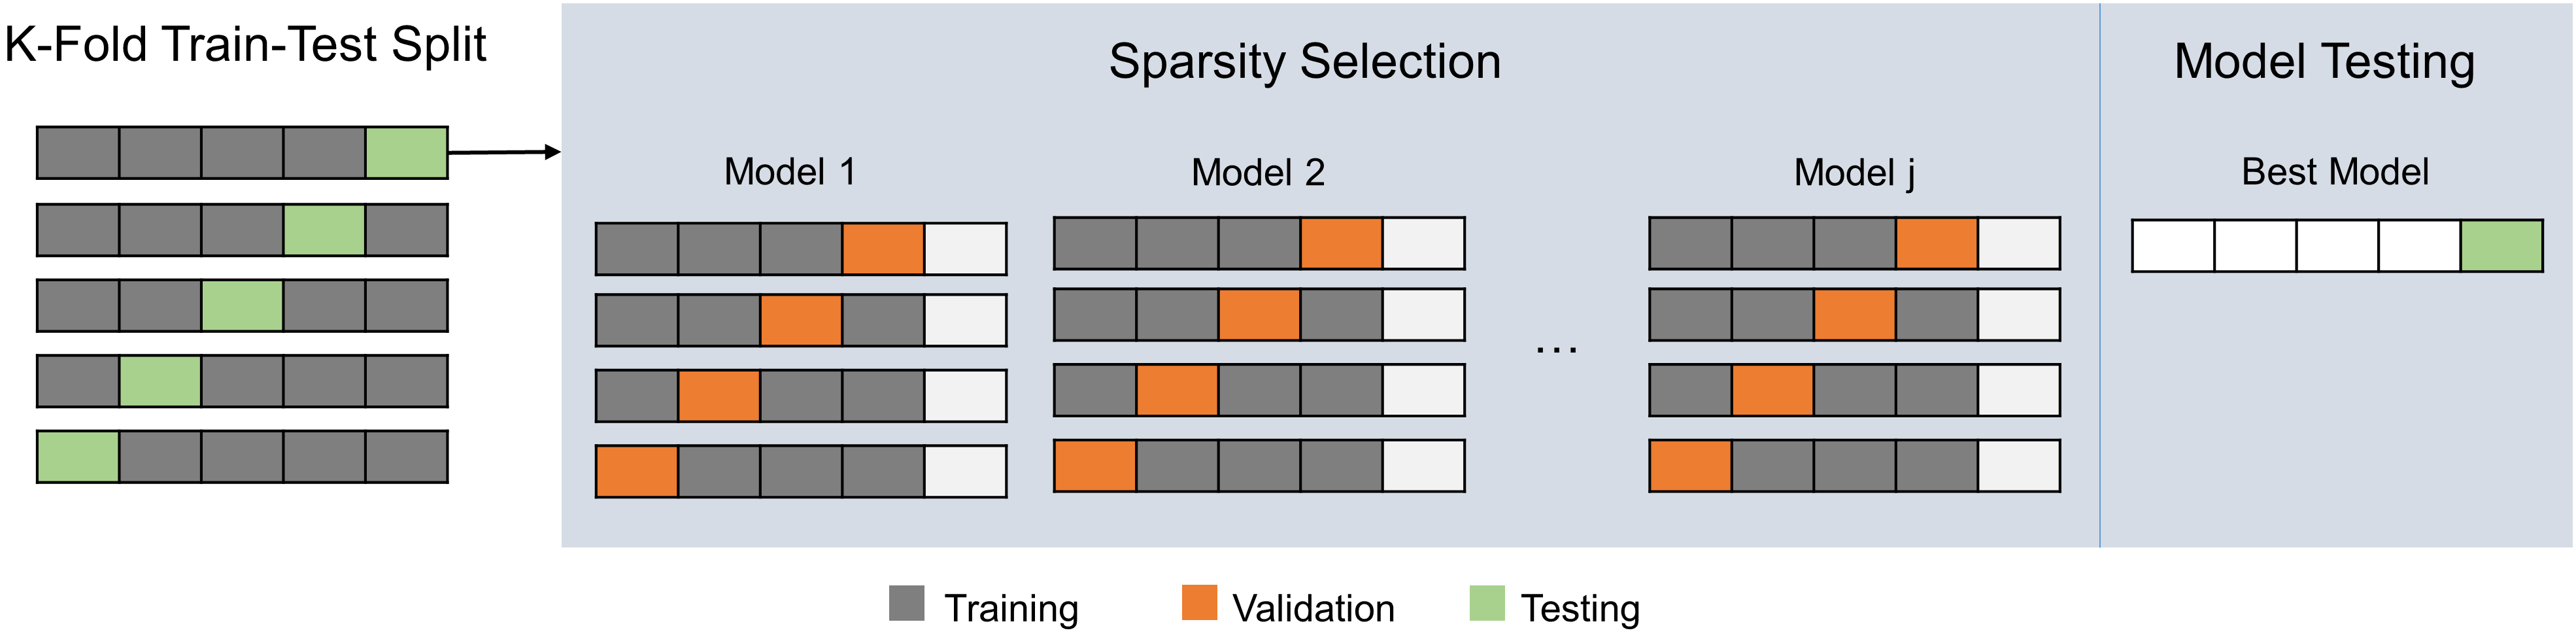
\includegraphics[width=0.8\textwidth]{study2/image/study2fig1.png}
	\caption{A diagram of the nested k-fold cross-validation with model selection.}
	\label{fig:study2:fig1}
\end{figure}

The number of latent components was determined by a preliminary analysis with no sparsity and calculated the explained variances for the two datasets (i.e., brain network correlations and questionnaire ratings). The explained variance increased with the number of components and growth stabilised at 10 components. We selected the number of components based on the point where the tangent stabilised. This led to a model of  4 components, and it accounted for a total of 78\% of the variance in connection strength and 29\% of the variance in the self-report data. Next, we determined the two coefficients for the L\textsubscript{1} penalty terms that was associated with the best model performance with 4 latent components. We searched for the best L\textsubscript{1} penalty values between 0.1 and 0.9 in 0.1 increments, which resulted in 81 set of parameters. For the nested K-Fold CV, we first separate the data into 5 consecutive folds after shuffling the data and retained one fold as the evaluation set (\(\mathit{N}\approx 50\)); the other four folds were used as the development set. The development set was further separated into 5 folds for parameter selection and each fold (\(\mathit{N}\approx 40\)) was used as the validation set once. The model was estimated on the training folds with all parameter sets, and after completion, we trained the model with the winning parameter on the whole development set and the finally tested the performance on the independent, unseen evaluation set. We selected the final parameters according to the best performance on the evaluation set across all folds of the outer CV loop (\cref{fig:study2:fig1}). This parameter set is used to train on the full development set and tested on the evaluation set. The parameter grid search and k-fold CV was conducted by the implementation in a Python library scikit-learn \cite<\url{http://scikit-learn.org/stable/}, version 0.18.2>{scikit-learn}.
The detailed algorithm for selecting the penalty values are presented in  \cref{appendix:kfold}: Nested K-Fold CV.

The model with the best test performance was selected as the final model. The final model’s sparsity coefficient are 0.8 (functional connectivity) and 0.5 (self-reports), and the out-of-sample explained variance was 48\%. We used the ensuing canonical vectors of the winning SCCA model to compute the latent component scores. There are two sets of canonical scores in a latent component, a weighted sum of variables forms the canonical vectors. For each latent component, we averaged the z-score of the canonical scores of the connection strength and NYC-Q as the combined scores. These scores described the summary of the experience with both the neural basis and the content reports.

\subsection{Test of component robustness}
\label{study2:method:robust}
After identifying the well performed components in compressing the brain-experience data, we examined the robustness of the four components in two different ways. The permutation test is a purely data-driven strategy that access the chance of discovering components in null samples. We also leveraged the brain-experience components to explain the cognitive functions, so that we can identify meaningful patterns by well-established cognitive measurements.

\subsubsection{Permutation test}
\label{study2:method:permute}
We used permutation testing to assess the robustness of the components identified through our analysis. We constructed a null distribution for each canonical component by holding the functional connectivity data in place and randomising the subject-wise order of self-reports data. This permutation scheme broke the link of individual differences in the dataset, therefore testing the robustness of the components in the hypothetical population. By calculating the false-discovery rate in the null distribution, we can conclude the possibility of discovering our components by chance with the given penalty coefficients. Hypotheses that are accepted with a 5\% level of significance. In the current analyses we adopt the permutation test with the FWE-corrected p-value by \citeA{Smith2015}
with data argumentation to increase the size of the resampling datasets to 1000. The four components were compared to the first sparse canonical correlation of the permuted sample. The low-rank components are more relevant that the rest, therefore we yield more conservative p-value by comparing to the first canonical correlation only. We performed 5000 permutation tests to get enough estimates for 4 decimal places.

\subsubsection{Group analysis}
\label{study2:method:manova}
To determine how patterns of unconstrained neurocognitive activity related to performance on the battery of cognitive tests, we conducted an independent statistical analysis on the identical subjects. A Type III multivariate multiple regression with Pillai's trace test was applied to 4 individual scores for each of the latent components describing experience from the SCCA  were the independent variables, and the original 8 measures of cognitive performance were the dependent variables that we hoped to described by the linear combination of the latent components. Pillai's trace test is considered to be the most powerful and robust statistic for general use \cite{Huberty2006}.
The p-values reported were based on Bonferroni correction. We also performed a principal components analysis (PCA) to identify the patterns of covariance among the 8 measures of cognitive performance and compressed the data. The relation between the principle score and the 4 brain-experience dimensions identified through SCCA was examined in a linear regression model with Pillai's trace test. The analysis was conducted in R (version 3.3.1).  The multivariate multiple regression was conducted in R (version 3.3.1) using function \texttt{Manova} in R package \texttt{car} (companion to applied regression, version 2.1-5).

\subsection{Code availability}
\label{study2:method:code}
The full analysis pipeline is freely available at \url{https://github.com/htwangtw/patterns-of-thought}.

% ==========================================================================================================

\section{Results}
\label{study2:results}

\subsection{Determining constituent category of experience}
\label{study2:results:cca}
We used Sparse Canonical Correlation Analysis (SCCA) to determine connectome-wide dimensions that describe common variance shared by descriptions of brain and experience. This took as input individual scores for the connections between each of the regions extracted from Yeo's 7 networks parcellation and the scores of each item of the New York Cognition Questionnaire (NYC-Q).

We applied SCCA with nested 5-fold CV as the model selection strategy. We obtained a model of 4 canonical components with penalty levels of 0.8 on the functional connectivity and 0.5 on the NYC-Q that indicated the best out-of-sample prediction on our data (see \cref{study2:method:ML:model}). The canonical correlations of the 4 latent components were 0.28, 0.19, 0.16, and 0.07. The latent components yielded by the best model are presented in \cref{fig:study2:fig2}. For the ease of presentation and interpretation, we summarised the components as network-network connectivity instead of 57-by-57 connectivity matrices. The heat maps describe the network-to-network correlations while the word clouds describe the loadings on the self-report items. The components in full and the heat map for the self-report items can be found in Online Supplementary Materials\footnote{Supplementary data related to this article can be found at \url{https://doi.org/10.1016/j.neuroimage.2018.04.064}}.

\begin{figure}
    \centering
    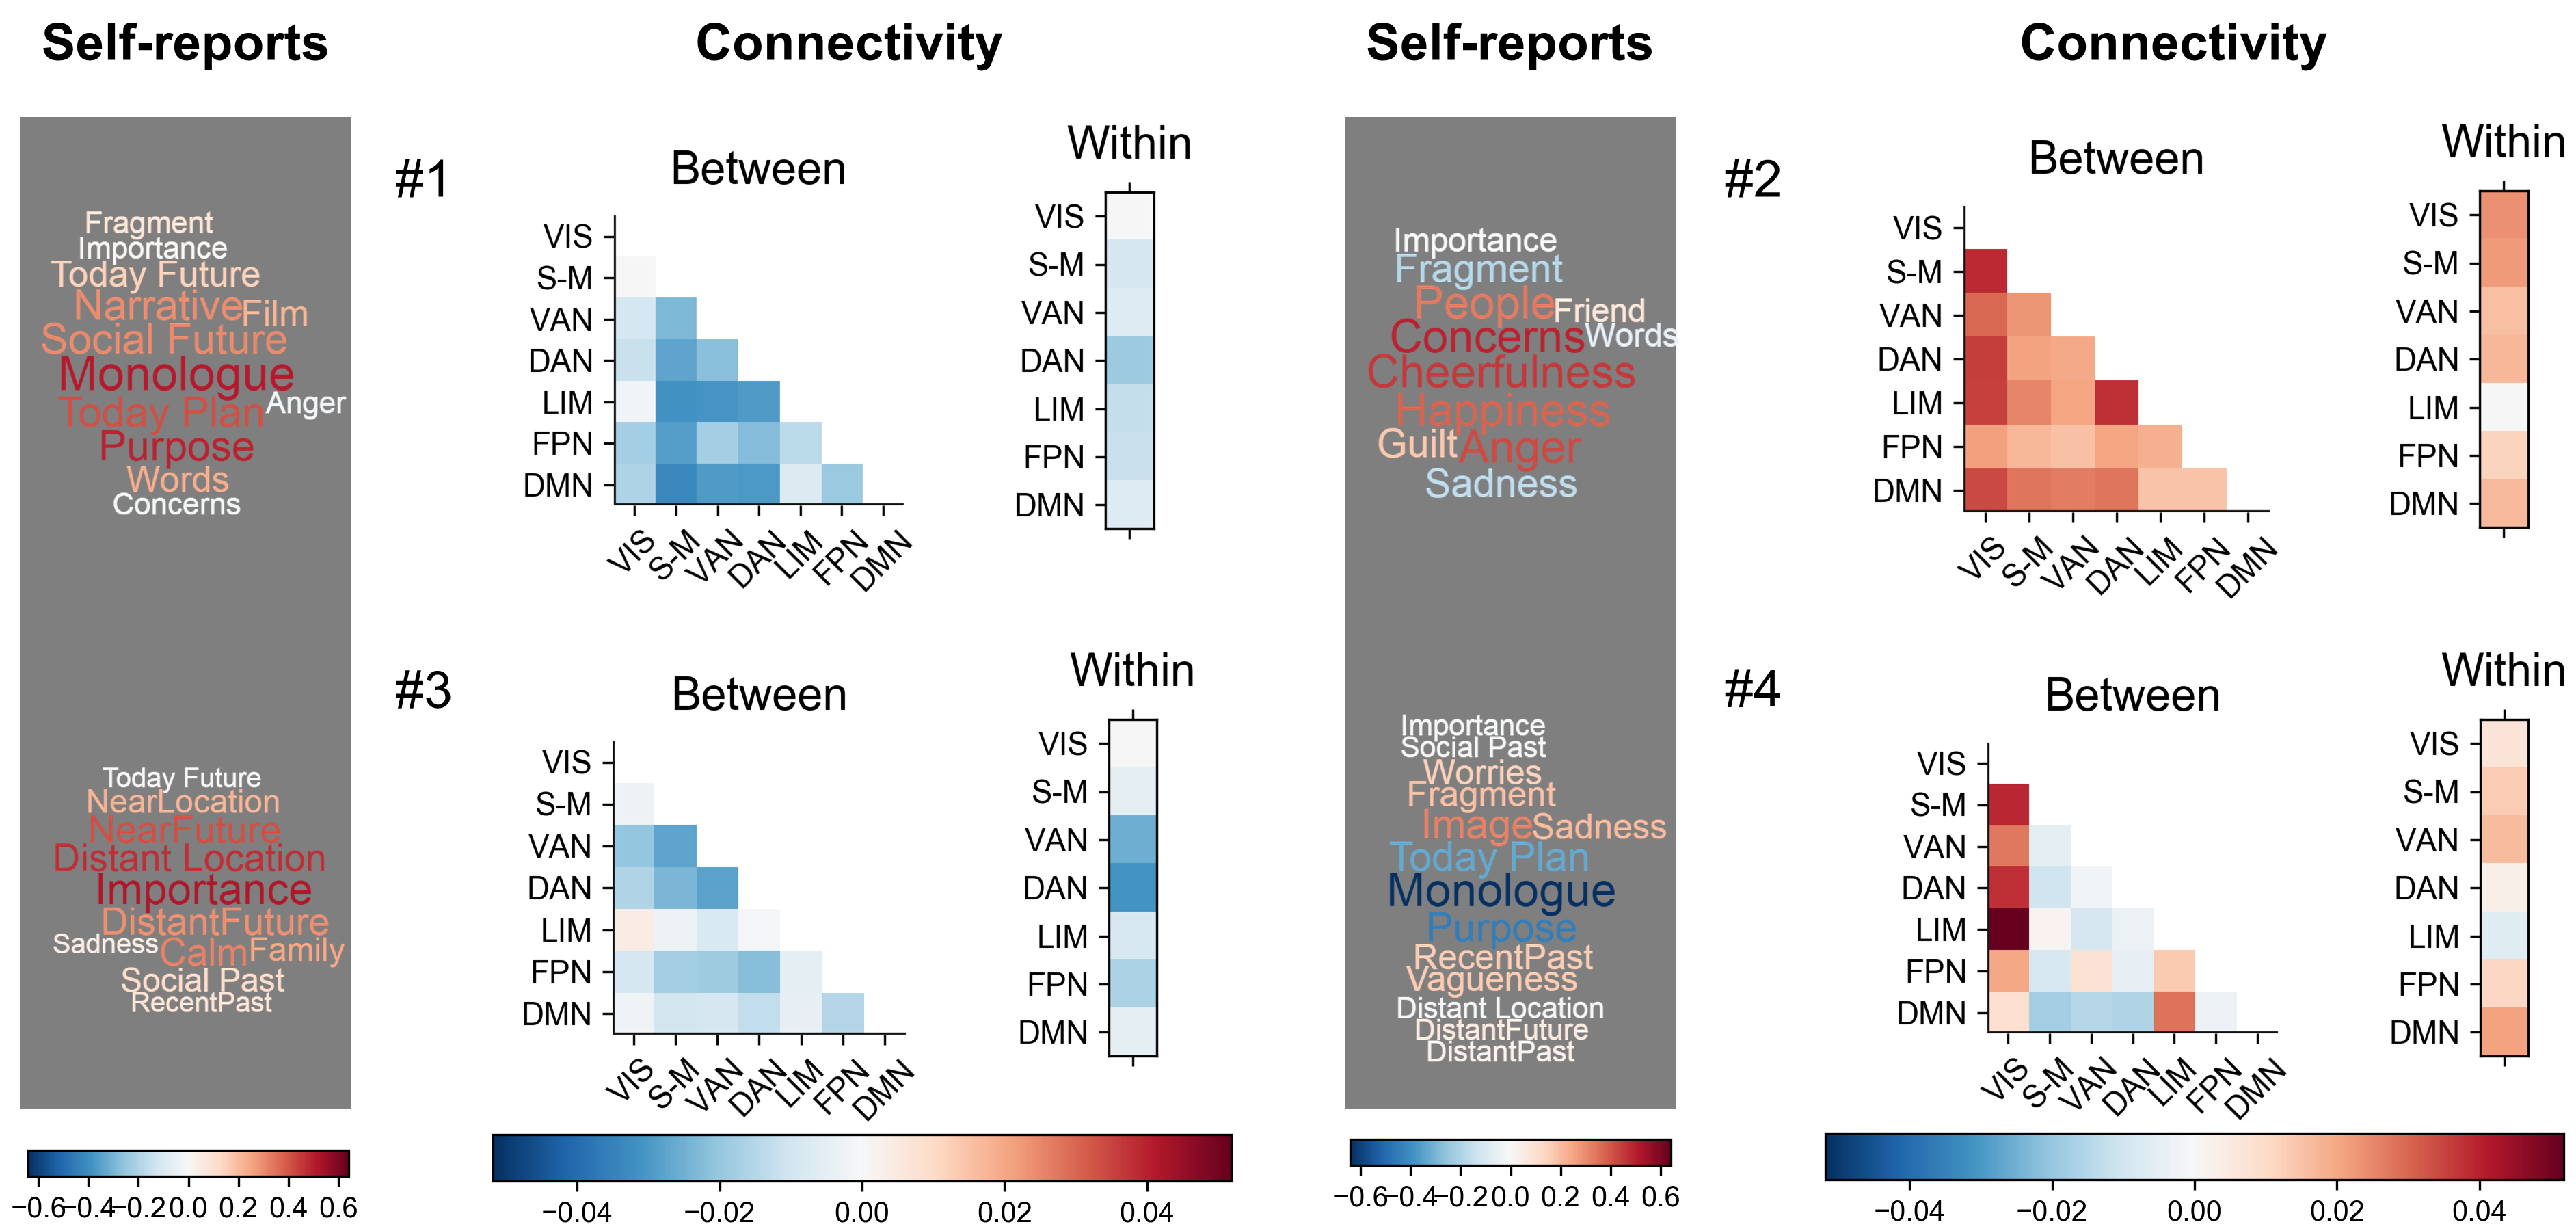
\includegraphics[width=0.8\textwidth]{study2/image/study2fig2.png}
    \caption{Unique neurocognitive dimensions of population variation revealed by sparse canonical correlation analysis of measures of whole brain connectivity and self-reported descriptions of ongoing experience.}
    \caption*{
    \footnotesize{
    The heat map describes the canonical variate of the network-to-network connectivity between different Yeo networks. The connectivity matrices describes the coefficients from the model, separated into within and between network relationships. The word clouds reflect the coefficients on the relevant self-report items. In both cases the colour bars indicate the magnitudes of the coefficients. A detailed version of the canonical variates and alternative presentation of the self-report coefficients can be found in  Online Supplementary Material Figure S1--S5
    }}
    \label{fig:study2:fig2}
\end{figure}

Component 1, describes patterns of reduced within network connectivity within all of the networks studied, with this pattern most prominent in the dorsal attention network. Between network connections are generally reduced, with the exception of visual to limbic. Sensorimotor was decoupled from all the other systems, and, in addition, the default and limbic were most decoupled from the attention networks. Experiential themes in Component 1 are dominated by themes related to deliberate planning with a verbal component (high loadings on `words', `monologue', `today-plan', `social-future', `purpose' and `deliberate'). We refer to this pattern of reports as reflecting thoughts with `purpose'.

Component 2 is dominated by relatively higher within and between network connections. Connectivity within each network was strong with the exception of the limbic network. Between network connections were stronger, with this pattern most apparent in the connections between limbic and ventral attention. In addition, the visual network was strongly correlated with the other networks. This component is dominated by emotional responses (high loadings on `anger', `guilt', `cheerfulness' and `happiness') and social content (`friends' and `people'). We refer to this pattern of reports as reflecting `emotional' experience.

Component 3 emphasises reduced connections both between and within networks. Within network connectivity is weakest for the dorsal and ventral attention networks. Edge-to-edge connections are low, with the ventral and dorsal attention and frontoparietal networks showing reduced correlations with each other as well as the visual and sensorimotor systems. This component was characterised by themes linked to personal `importance' with social temporal contents (`distant future', `near future', `social past', `family' and `recent past'). We refer to this pattern of reports as reflecting `personal importance'.

Component 4 has the most heterogeneous pattern of within and between network connectivity. It is associated with stronger connections within networks with the exception of the limbic system. In addition, the visual system was strongly connected to all other networks, with this pattern most apparent for the limbic network. In contrast, lower network-to-network connectivity was observed between the default mode and sensorimotor and attention networks. This component is characterised by experiential patterns reflecting a modality difference in experience, with the highest loadings on `images' and lowest on `inner monologue'. We refer to this pattern of reports as describing `modality'.


\subsection{The relationship between neuroexperiential components and cognitive functions}
\label{study2:results:manova}
Having documented four neurocognitive dimensions, we next examined the robustness of the components using two complementary approaches. We first used a permutation test to identify the chance of discovering components in null samples as employed by Smith and colleagues (2015). The top three components passed the permutation test and the \nth{4} component showed variance that was similar to that produced in a null sample
(Component 1: \(\mathit{p} = 0.0002\),
Component 2: \(\mathit{p} = 0.0010\),
Component 3: \(\mathit{p} = 0.0204\),
Component 4: \(\mathit{p} = 0.998\),
\(\alpha = 0.05\)).
This analysis suggests that Components 1--3 are unlikely to have occurred by chance. Component 4 may be a Type \rom{2} error and so we discuss this component in only a limited manner moving forward.
Our next test of the robustness of our components is whether they explained unique patterns of expertise in our battery of cognitive tasks. We used multiple multivariate regression model in which performance on the battery of selected tasks was the dependent variables and the individual scores for each of the canonical components describing experience from the SCCA were the independent variables. In this analysis two of the four canonical components described significant variance in our battery of tasks at multivariate level: 
Component 1 
(\(\mathit{F}(8, 246) = 2.21\),
\(\mathit{p} = .027\),
\(\mparetasquared = .067\))
 and Component 3 
(\(\mathit{F}(8, 246) = 2.56\),
\(\mathit{p} = .024\),
\(\mparetasquared = .068\)).

\begin{figure}[p]
    \centering
    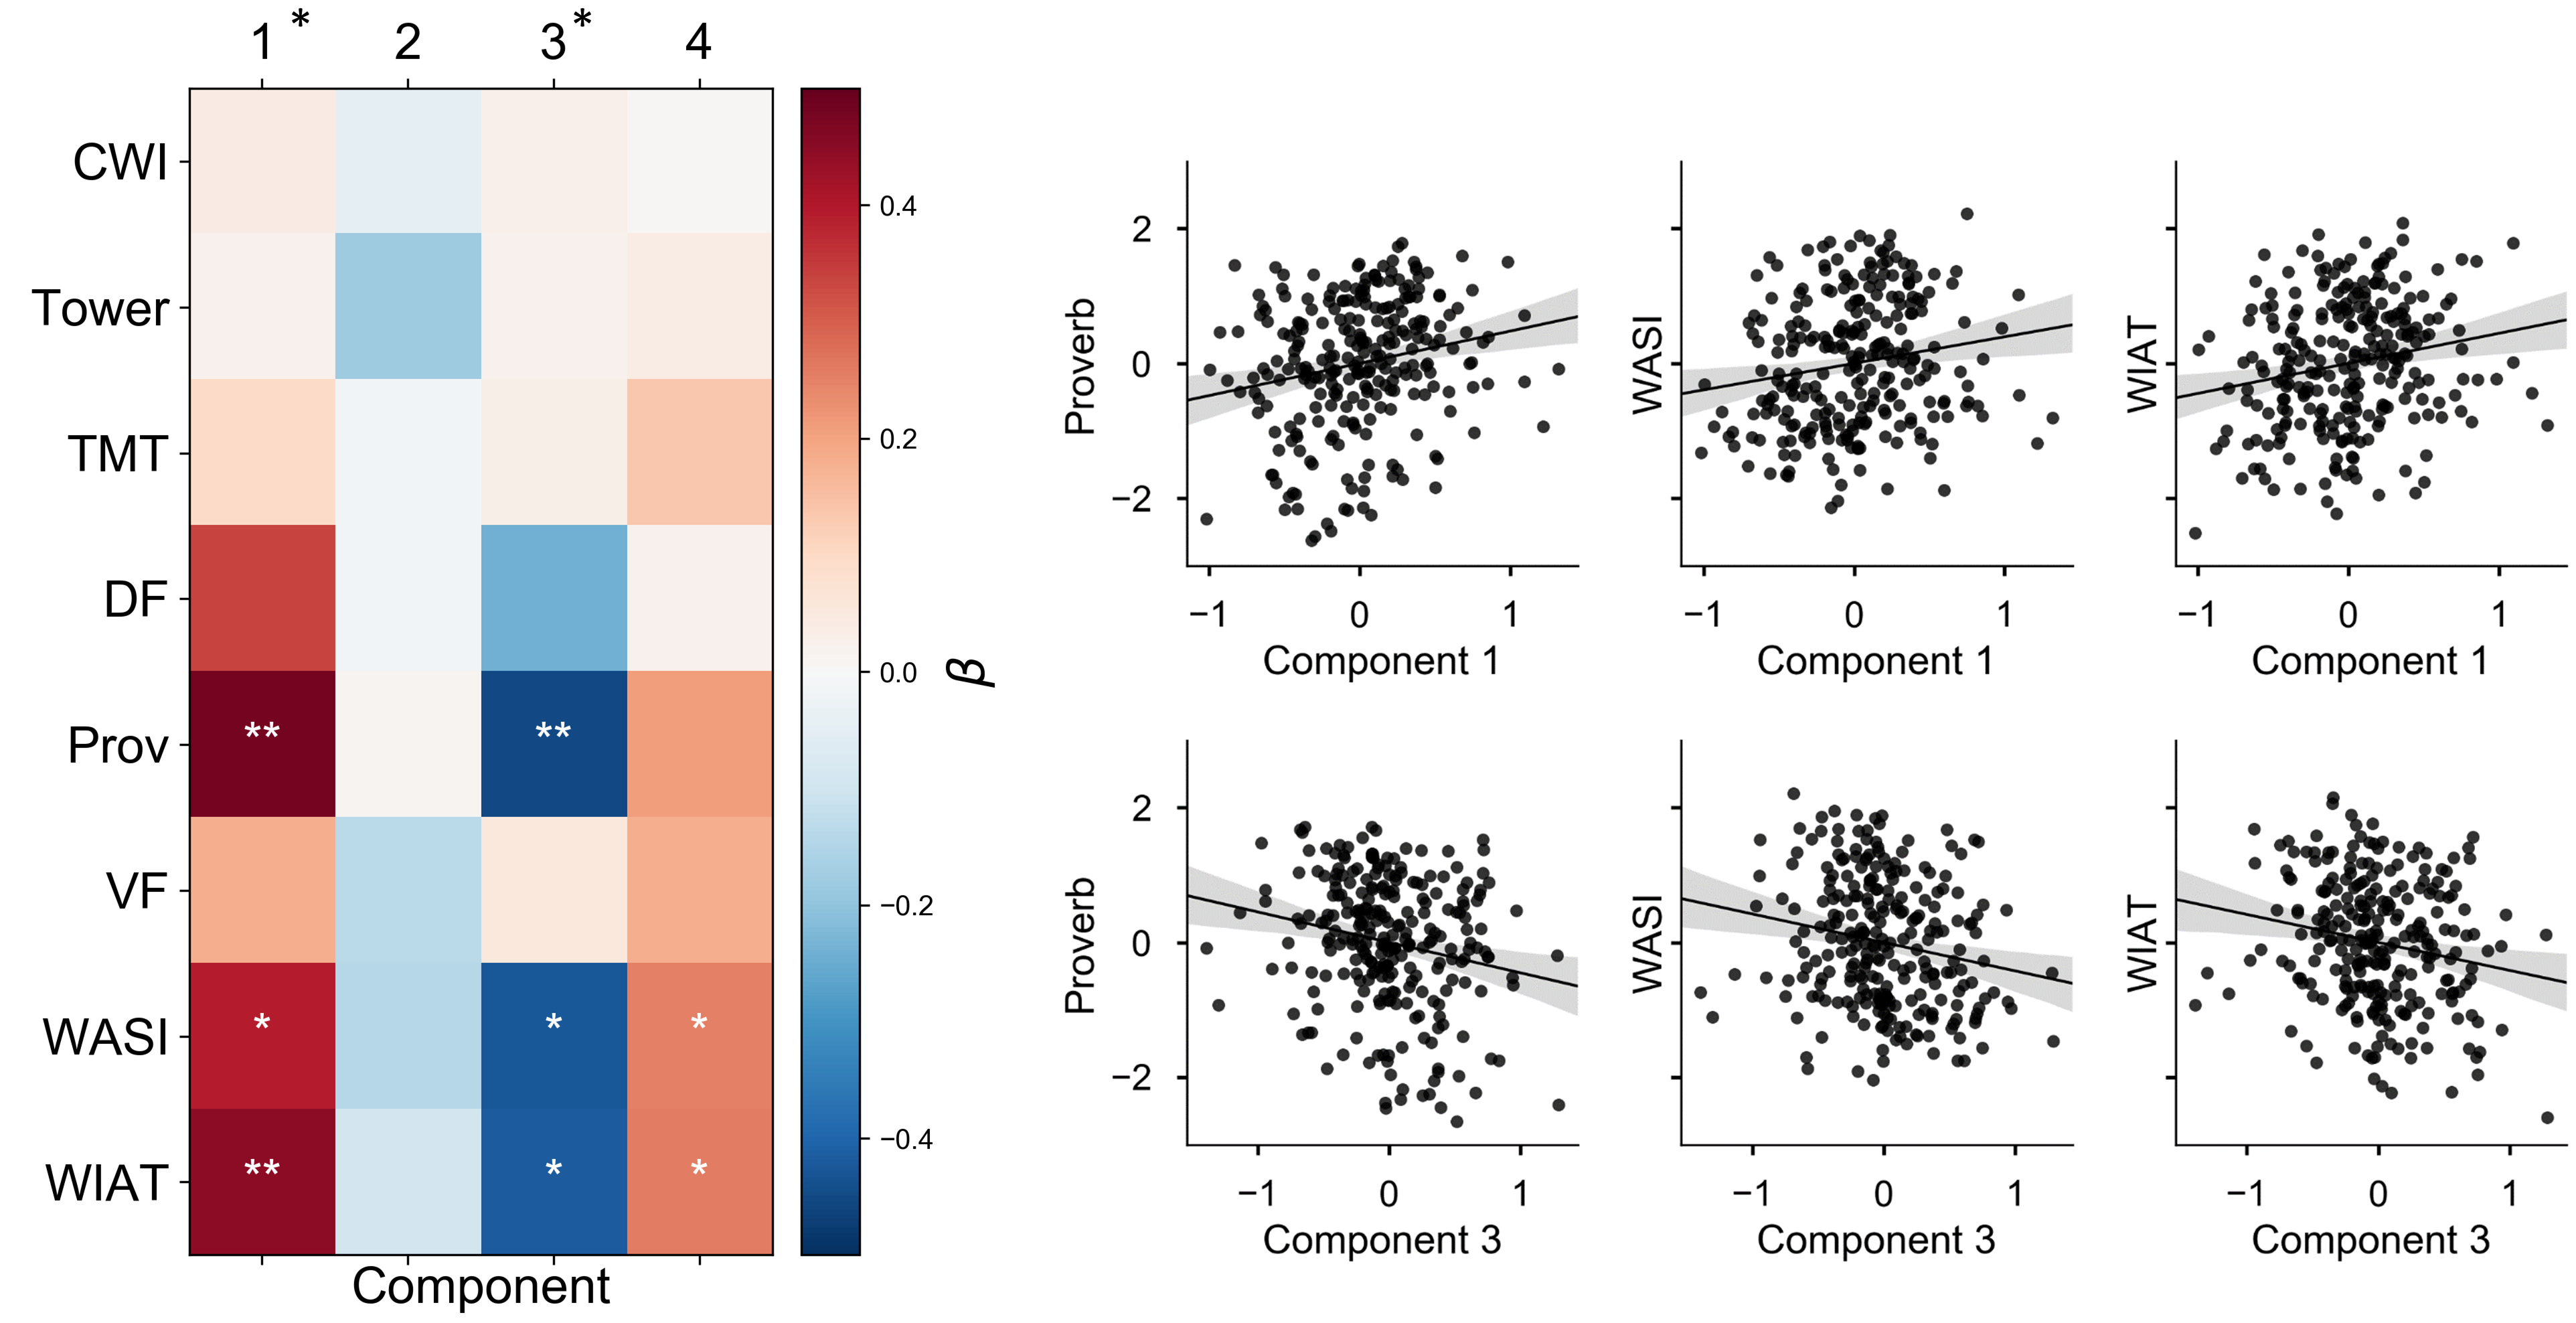
\includegraphics[width=0.7\textwidth]{study2/image/study2fig3.png}
    \caption{The relationship between the different neural-cognitive components and the measures assessed in the cognitive battery.}
    \caption*{
    \footnotesize{
    The components 1 and 3 were significant at the multivariate level determined by multiple multivariate regression, indicated by the asterisk outside of the heat map. The cells with asterisk(s) indicates the significant results from the univariate test (bonferroni corrected) and the parameter estimates for each variable. CWI: Colour-word interference, DF: Design fluency, Pro: Proverbs, TOW: Tower of London, TMT: Trail making task, VF: Verbal Fluency, WASI: Wechseler Adult Intelligence Test, WIAT: Weschler Individual Attainment Test. P-value significant codes:  0 `***' 0.001 `**' 0.01 `*' .}
    }
    \label{fig:study2:fig3}
\end{figure}

\begin{figure}[p]
    \centering
    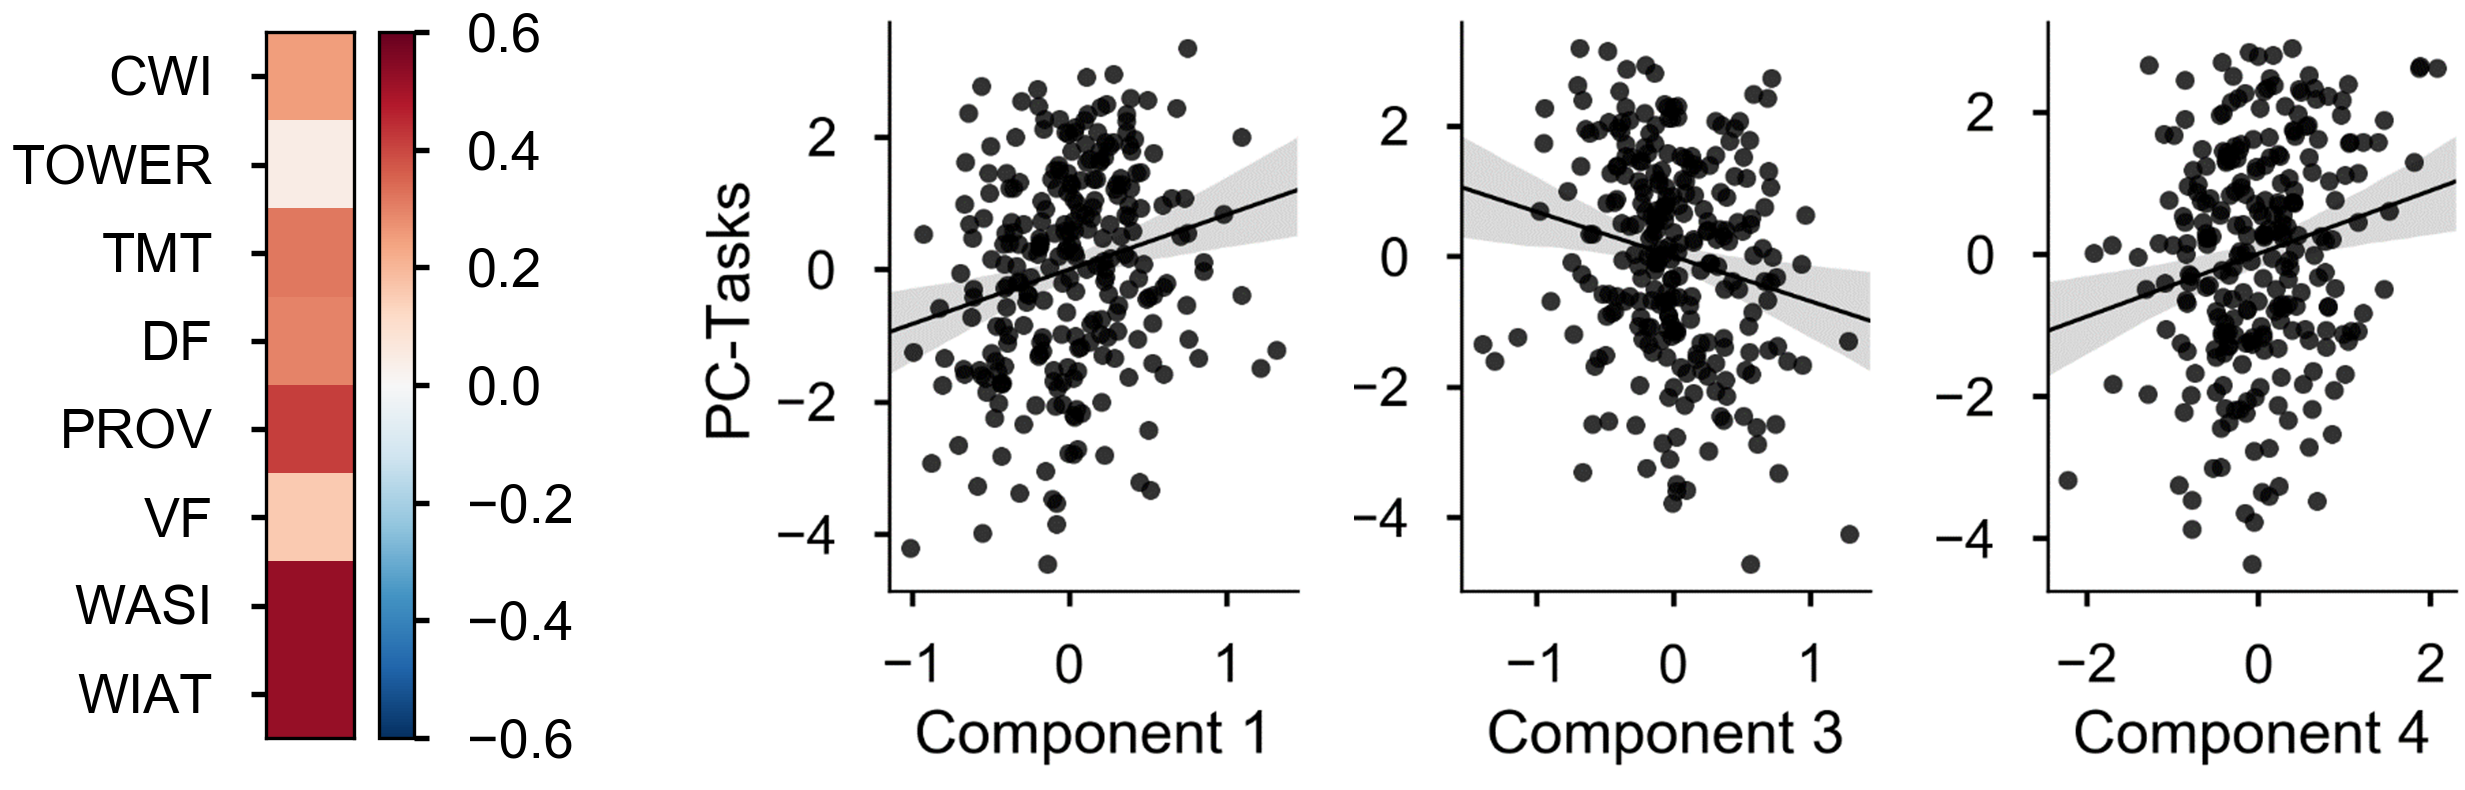
\includegraphics[width=0.7\textwidth]{study2/image/study2fig4.png}
    \caption{The principle component and its relationship to the different neurocognitive components.}
    \caption*{
    \footnotesize{The heat map describes the principle component of the task battery, and the scatter plots describe the association with the components identified in our study. Component 1 and 3 passed the permutation test for component robustness significantly contributed in explaining the principle component of the task. Component 4 showed a significant contribution in the regression model, but it did not pass the permutation test. The related results should be treated cautiously.}
    }
    \label{fig:study2:fig4}
\end{figure}

In the univariate results of the significant component, Component 1 was linked to good performance in proverb test 
(\(\mathit{b} = 0.48\),
\(\text{95\% CI} = [0.191  0.766]\),
\(\mathit{t}(251) = 3.27\),
\(\mathit{p} = .006\)) 
and both fluid intelligent tests WASI
(\(\mathit{b} = 0.39\),
\(\text{95\% CI} = [0.111 0.677]\),
\(\mathit{t}(251) = 2.74\),
\(\mathit{p} = .033\)) 
and WIAT
(\(\mathit{b} = 0.45\),
\(\text{95\% CI} = [0.167 0.724]\),
\(\mathit{t}(251) = 3.15\),
\(\mathit{p} = .009\)). Component 3 showed a reversed pattern of the cognitive functions related to Component 1: proverb test 
(\(\mathit{b} = -0.45\),
\(\text{95\% CI} = [-0.176 -0.727]\),
\(\mathit{t}(251) = -0.14\),
\(\mathit{p} = .007\)); WASI 
(\(\mathit{b} = -0.42\),
\(\text{95\% CI} = [-0.151 -0.693]\),
\(\mathit{t}(251) = -3.10\),
\(\mathit{p} = .012\)) and WIAT 
(\(\mathit{b} = -0.41\),
\(\text{95\% CI} = [-0.148 -0.682]\),
\(\mathit{t}(251) = -3.06\),
\(\mathit{p} = .012\)). 
The relationships between the neurocognitive dimensions and the pattern of relationships on the full cognitive battery and the adjusted variable scatter plots of the significant results are summarized in the form of a heat map in \cref{fig:study2:fig3}.

Finally, we performed a simple principle component analysis on the eight task measures to explore the associations between experience and the structure of the laboratory data. The aim of this analysis was to see if the pattern retrieved from the univariate level in the previous multiple multivariate regression was related to the internal structure of the data. Component selection was determined based on the scree plot, and we accepted one component explaining 39\% of the variance. The principle component loaded on the intelligence measures and the proverb test. We fitted a linear model to this data to understand the relationship to the four canonical components. The results are reported in \cref{fig:study2:fig4}. The overall linear model was significant 
(\(\mathit{F}(4, 253) = 5.43\),
\(\mathit{p} = .00003\)). In the linear regression model, Component 1 
(\(\mathit{b} = 0.82\),
\(\text{95\% CI} = [0.36 1.29]\),
\(\mathit{t}(253) = 3.5\),
\(\mathit{p} = .001\)) showed significant contribution to explaining the task principle component. Component 3 showed a negative correlation to the task components 
(\(\mathit{b} = -0.69\),
\(\text{95\% CI} = [-1.13 -0.24]\),
\(\mathit{t}(253) = -3.04\),
\(\mathit{p} = .003\)). The relationships between tasks and the neurocognitive components here were similar to the ones uncovered by the multiple multivariate regression. In this analysis Component 4 
(\(\mathit{b} = 0.442\),
\(\text{95\% CI} = [0.16 0.72]\),
\(\mathit{t}(253) = 3.09\),
\(\mathit{p} = .002\)) showed a significant contribution in the regression model, but it did not pass the permutation test of robustness (\(\mathit{p} = 0.998\)). The related results should be treated cautiously. Together with our prior analysis, these results suggest that Components 1 and 3 are the most robust components identified in our study.

% ==========================================================================================================

\section{Discussion}
\label{study2:discussion}
We set out to describe different modes of neurocognitive patterns derived through the simultaneous decomposition of whole brain connectivity data with self-reports of ongoing experience. We used a whole brain parcellation that describes cortical function in seven independent networks \cite{Yeo2011}.
We combined this data with self-reports of the experience of our participants at rest, using a multivariate approach that allows for the possibility of many-to-many mappings between neural patterns and ongoing cognition. Our analyses identified four stable canonical components, describing unique dimensions of neural-experiential variation. Permutation testing demonstrated the statistical robustness of Components 1-3. Furthermore, two components (1 and 3) described independent patterns of performance in a battery of commonly used cognitive measures. This association with cognitive performance that establishes a source of independent validity for these neurocognitive components since they are related to independent measures of cognitive performance. We next consider the fit between the dimensions produced by our analysis and theoretical views of unconstrained neurocognitive processing.

We found evidence broadly consistent with contemporary representational accounts of unconstrained processing. The neural patterns described by Component One reflect a pattern of reduced correlation between regions with links to memory and representation (e.g. limbic, default mode) from those with links to external behaviour (e.g. visual and sensorimotor cortex and attention networks). This pattern was associated with experiences characterised by a sense of purposefulness, and with verbally mediated content that was social and temporal in nature. Participants high on this dimension were proficient at generating abstract semantic links and performed well on measures of reasoning and intelligence. Together the features of Component One support the hypothesis that the functional decoupling of systems important for memory and representation are important for aspects of unconstrained cognition \cite{SmallwoodFrontiers2013}.
This capacity may arise from the topographical organisation of the cortex, in which neural systems that can take on more transmodal properties tend to be located in regions that are more distant in functional and structural terms \cite{Buckner2013,Margulies2016,Mesulam1998}.
This spatial location may allow neural signals in these regions to take on properties that are discrepant from the neural signal more closely tethered to inputs describing the external world \cite{Buckner2013,Friston2013}.
The pattern identified by Component One, therefore, may reflect a pattern of population variation describing the hypothesised role of functional decoupling of memory and representational systems plays in the generation of more abstract aspects of human cognition \cite{Margulies2016,Mesulam1998}.
Importantly, in our prior work, limbic and default mode networks were the most distant in functional connectivity terms from unimodal systems \cite{Margulies2016}.
Our data also highlights neural patterns that capture the hypothesised influence of attention and control on ongoing thought \cite{McVay2009}.
Component 3 highlights links between reduced connectivity within attention and control systems and patterns of thought that emphasise personal importance. This is associated with worse performance on measures of intelligence and reasoning. The combination of a focus on personally important themes linked to poor performance on measures of general aptitude, captures the hallmark psychological features of the `current concerns--executive-failure` accounts of ongoing thought \cite{McVay2009}.
This view suggests that failures in attentional control lead to highly personally relevant cognition to intrude into ongoing thought, leading to lapses in task performance. Importantly, the neural pattern described by this component emphasises dysregulated connectivity both within and between networks implicated in attention and control by task-based studies \cite{Duncan2010}.
Our prior work established that spontaneous mind-wandering is linked to cortical thinning within regions linked to attention and control, such as the intra-parietal sulcus \cite{Golchert2017}.
Spontaneous mind-wandering has been linked to worse cognitive control \cite{Robison2018},
as well as showing stronger links with attention related problems, including ADHD \cite{SeliADHD2015}.
Together with these prior studies, our data suggests that population variation in the intrinsic neural functioning within networks with an established role in external task performance captures the hypothesised contribution of executive-failure to patterns of ongoing thought.

The method of decomposition used in the current study also highlighted patterns related to affective processing and the modality of the experience that are similar to those seen in our prior work that applied principal components analysis (PCA) to self-reported data only. Component Four places experiences with visual features (`images') in opposition to experiences with verbal features (`monologue'), capturing dissociations between visual and verbal thinking observed in our prior studies \cite{Konishi2015,Medea2016,Smallwood2016}.
The accompanying neural pattern were associated with higher connectivity between the visual network with other networks, in particular the limbic system. It is important to note that our permutation analysis failed to validate this component, so despite its association with task performance using the PCA analysis it should be treated with relative caution. Component Two loads on emotional experiences (`cheerfulness', `anger', `guilt' and `happiness') with the exception of those that are unhappy (`sad'). In neural terms this component was characterised by high levels of connectivity, however, unlike Component Four, this was highest between limbic and ventral attention networks. This pattern of coupling is consistent with accounts that emphasise interactions between saliency and limbic systems in affective processing \cite{Touroutoglou2012}.
In the case of Component Two permutation testing indicated this component was likely to be robust in statistical terms, however, we did not observe associations with task performance. As with Component Four, interpretations of Component Two should be made with caution in lieu of more empirical work.

Before closing it is worth considering several important limiting factors of our study. We focused on patterns of population variance in unconstrained neurocognitive processing that were measured once in each individual. Our study, therefore, cannot separate the influences of state and traits on our observed components. Treating patterns of unconstrained processing as a trait is common in both the psychological \cite{McVay2009,SmallwoodCC2013}
and neural domains \cite{Smith2015}.
Nonetheless, it remains an open question how consistent these components will be across individuals over time, as well as which aspects may be better described as traits. Importantly, by its very nature there are dimensions of experience that our study cannot adequately address. We cannot, for example, identify brain-experience associations that are highly dynamic in nature and in particular those that change rapidly within an individual. Insight into this issue could be achieved by a focus on dynamic rather than static connectivity \cite{Kucyi2017}.
For example, the application of techniques such as sliding window analysis \cite{Chang2010}%(Chang \& Glover, 2010)
or Hidden Markov models \cite{Vidaurre2017}
to fMRI could provide information that would complement our analyses. However, it may also be more important to examine these across multiple sessions within the same individuals, as this would also make it most possible to dissociate state from trait related influences on neural activity \cite{Mueller2013}. %(Mueller et al., 2013).
There are also types of experience that may be difficult to assess using the measure of retrospective experience sampling we have employed \cite{SmallwoodSchooler2015}.
For important features of experience, such as whether it has evolving features \cite{Mills2018},
or when the participant is unaware of the content of their experience \cite{Schooler2002}%(Schooler, 2002),
these experiential features may be best assessed using experience sampling techniques that capture momentary elements of experience \cite{Smallwood2013}. %Smallwood 2013 Psychological Bulletin

There are a number of methodological improvements that could enhance future studies of brain-experience association. A recent benchmark study by \citeA{Ciric2017} %(Ciric et al., 2017)
shows that scrubbing can improve the performance of resting state analyses. Regarding to the analysis pipeline, we gained hyper-parameters and best model with nested-CV an approach that can help prevent overfitting \cite{BzdokYeo2017}. %(Bzdok & Yeo, 2017).
There are also alternative ways that could provide better tests of the robustness of the components we identified. We assessed the validity of the components in three different ways; (i) with a data-driven, non-parametric permutation test \cite{Smith2015}%(Smith et al., 2015)
that establishes the statistical validity of the identified components and (ii) by establishing the relationship between the laboratory cognitive measures and (iii) by consideration of their links with contemporary theoretical accounts of ongoing cognition. In our study, Components 1 and 3 were statistically significant in both cases and fitted well with contemporary accounts of ongoing cognition. Accordingly we place encourage readers to focus on these patterns from our data. There are alternative strategies that could help validate the robustness of patterns of brain-experience association. One approach could be to compare the relationship between multiple sessions within the same individual \cite{Poldrack2015} %(Poldrack et al., 2015)
and to have a larger sample that would allow the reproducibility of these results through a formal split-half validation procedure. To achieve this latter aim for future studies, we have placed the questionnaire measure used in this study along with an example self-report collection task on GitHub at the following address: \url{https://github.com/htwangtw/restingstate_thoughtreports}.
We encourage interested investigators to apply these measures in their resting-state investigation and to also upload the resultant data onto open fMRI. These studies could be used in conjunction with the openly access data used in this study to enable future investigations the opportunity to cross validate experiential analyses in a more sophisticated manner than we have been able to achieve in this study. The analysis pipeline of the current study can be further unified into one frame work that benefits from both validation strategies. We can include the number of components along with penalty coefficients in the hyper-parameters determined in the CV process, or determine the best penalty terms with the first component. The permutation test will then identify the reliable components occurring above chance level. After all the data-driven component selection, we can examine the survived components through their relations with well-documented cognitive measures and conclude the meaningful patterns. Finally, it is likely that our measure of ongoing thought lacks important questions regarding the content of experience. It will be important, therefore, in the future to examine the relationships of the type described in this study with a more exhaustive description of ongoing experience. We hope that by publishing our questionnaire collection task in a GitHub repository we will be able to harness the power of the broader community to help generate and test plausible questions for use in future studies.

% ==========================================================================================================
